\documentclass[11pt]{article}
\usepackage{hyperref}
\usepackage{amsthm}
\usepackage{amsmath}
\usepackage{amsfonts}
\usepackage{tikz}
\usepackage{ wasysym }
\usepackage{fancyvrb}

\newtheorem{example}{Example}


\author{Group 3:  Hannah Jensen, Nicholas Jacob}
\title{Homework 1 Advanced Analytics and Metaheuristics}

\begin{document}
\maketitle
%{\Large
%%Change Document name to: Graded Homework 1\_Jacob\_Nicholas
%\noindent NAME:  Nicholas Jacob\\ 
%STUDENT ID: \# 113578513\\
%HOMEWORK NUMBER: 1\\
%COURSE: DSA 5113 Advanced Analytics and Metaheuristics\\ 
%SECTION: ONLINE\\SEMESTER: Spring 2024\\
%INSTRUCTOR:  DR. Charles Nicholson\\
% SCORE:}
%
%\newpage
\begin{enumerate}
\item To examine this story, we create a table:  
\begin{center}
\begin{tabular}{c|c|c|c}
Baby Yoda Tells Truth&gurump = yes&pvlork = yes& Possible\\ \hline
T&T& T&N\\
T&T&F&N\\
T &F &T&N\\
T&F&F&N\\
F&T&T&N\\
F&T&F&Y\\
F&F&T&Y\\
F&F&F&N

\end{tabular}
\end{center}

I will assume that a sinister lying creature always lies (even though we know this too not be true eg. politicians).  

Let's examine each with our information.  We were told that the words meant yes or no so we assume that they cannot both mean the same thing.  This eliminates half of our truth table.  Next, we see that if Jedi would tell the truth, the statement cannot be.  You would not answer yes to a wrong question.  Similarly you cannot have the third entry either as you will tell the truth.  We move on to sith liars.  If gurump means No and asked if it means yes, a liar would reply in the affirmative.  This means the logic on the sixth one is possible.  We see the seventh is also possible.  Since gurump is yes and the creature lies, we would answer no or pvlork.  Thus we see that Baby Yoda is a liar.  We cannot however determine the meaning of gurump and pvlork.


\item I am going to state the problem here
\begin{quote}
A portfolio manager in charge of a bank portfolio has \$10 million to invest. The
securities available for purchase, as well as their respective quality ratings, maturities, and yields, are shown
in Table

{\tiny
\begin{tabular}{c|c|c|c|c|c|c}
Name & Type & QS Moody's & QS Banks& Years to M & Yield to m& After-tax yield\\\hline
A& Municipal& Aa &2& 9& 4.3\% &4.3\%\\
B& Agency& Aa& 2& 15& 5.4& 2.7\\
C& Government& Aaa &1 &4 &5.0 &2.5\\
D &Government &Aaa& 1& 3& 4.4& 2.2\\
E& Municipal &Ba &5 &2 &4.5 &4.5
\end{tabular}}

The bank places the following policy limitations on the portfolio manager’s actions:
\begin{enumerate}
\item Government and agency bonds must total at least \$4 million.
\item  The average quality of the portfolio cannot exceed 1.4 on the bank’s quality scale. (Note that a low
number on this scale means a high-quality bond.)
\item  The average years to maturity of the portfolio must not exceed 5 years.
\end{enumerate}

\begin{enumerate}
\item Assuming that the objective of the portfolio manager is to maximize after-tax earnings and that the tax rate is 50 percent, what bonds should he purchase? 
\item If it became possible to borrow up to \$1 million at 5.5 percent before taxes, how should his selection be changed?
\end{enumerate}
\end{quote}

\begin{enumerate}
\item 
We'll start by stating the objective function, the return on investment after taxes:
\[
P(\vec x) = 0.043x_A + 0.027 x_B + 0.025 x_C + 0.022 x_D + 0.045 x_E
\]
This is the function that we wish to maximize.

Next we examine each of the constraints.
There is a total of 10 million to invest
\[
\sum x_i \leq 10 000 000
\]

  We need a total of at least 4 million in government and agency bonds so
\[
x_B + x_C+x_D \geq 4 000 000
\]
Then we want the average on the banks quality scale to not exceed 1.4 so
\[
\frac{2x_A +2x_B +x_C + x_D +5x_E}{\sum x_i} \leq 1.4
\]
We need to make this linear for AMPL (I learned after only a few minutes of face to keyboard)
\[
2x_A +2x_B +x_C + x_D +5x_E -1.4\sum x_i \leq 0
\]
Which can be simplified to (but was not required in AMPL) 
\[
0.6 x_A + 0.6 x_B -0.4 x_C -0.4 x_D +3.6 x_E \leq 0
\]
Lastly we wanted the average years to maturity to be less than 5 so 
\[
\frac{9x_A +15x_B +4x_C + 3x_D +2x_E}{\sum x_i} \leq 5
\]
This simplifies to 
\[
4x_A +10x_B -x_C -2 x_D -3x_E\leq 0
\]
With all of this we code it into AMPL and arrive at the output: 

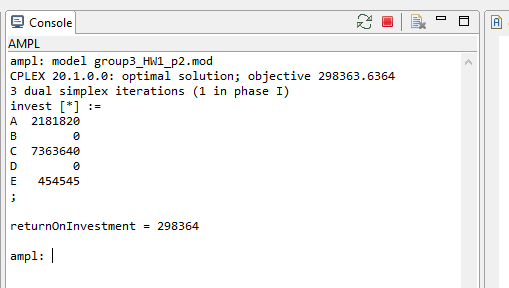
\includegraphics{outputp2a.png}

\item 
For the second part of the problem, we add the additional condition that we can take out a loan of up to 1 million at 5.5\%.  This will change our objective function in significant ways and add an extra variable $x_{loan}$.  We examine the new objective, we will use the before tax rates and recognize that Municipal bonds grow tax free.  We also note that our total interest is subtracted from our tax liability
\begin{eqnarray*}
z =& interestEarned - interestPaid - taxesPaid\\
=& \sum_i BeforeTaxRates_i x_i-0.055 x_{loan} - 0.5(taxableIncome)\\
=& 0.043x_A + 0.054 x_B + 0.05 x_C + 0.044 x_D + 0.045 x_E -0.055 x_{loan}\\
&\phantom{    something something}-0.5\left(0.054x_B +0.05x_C +0.044 x_D -0.055x_{loan}\right)
\end{eqnarray*}
The total amount invested must also change
\[
\sum x_i \leq 10 000 000 + x_{loan}
\]
Of course there are the restrictions on the loan too
\[
0\leq x_{loan}\leq 1 000 000
\]
The rest of the constraints remain unchanged.  Running it through AMPL arrives at the solution:

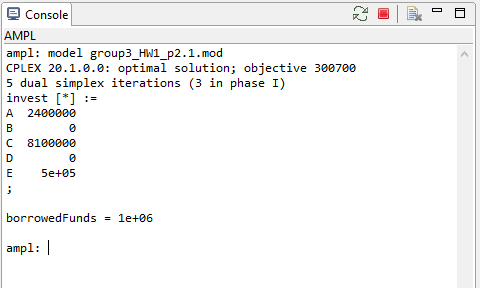
\includegraphics{outputp2b.png}

\end{enumerate}

\item I am going to state the problem here:

\begin{quote}
This exercise starts with a two-variable linear program similar in structure to the one of Sec-
tions 1.1 and 1.2, but with a quite different story behind it.
\begin{enumerate}
\item You are in charge of an advertising campaign for a new product, with a budget of \$1 million.
You can advertise on TV or in magazines. One minute of TV time costs \$20,000 and reaches 1.8
million potential customers; a magazine page costs \$10,000 and reaches 1 million. You must sign
up for at least 10 minutes of TV time. How should you spend your budget to maximize your audience? Formulate the problem in AMPL and solve it. Check the solution by hand using at least one of the approaches described in Section 1.1.

\item It takes creative talent to create effective advertising; in your organization, it takes three
person-weeks to create a magazine page, and one person-week to create a TV minute. You have
only 100 person-weeks available. Add this constraint to the model and determine how you should
now spend your budget.
\item Radio advertising reaches a quarter million people per minute, costs \$2,000 per minute, and
requires only 1 person-day of time. How does this medium affect your solutions?
\item How does the solution change if you have to sign up for at least two magazine pages? A maximum of 120 minutes of radio?
\end{enumerate}
\end{quote}

\begin{enumerate}
\item We begin by stating the objective function to maximize, eyeballs:
\[
z = 1.8 x + 1y
\]
Where $x$ is minutes of TV time, $y$ is pages in a magazine and $z$ is million viewers.  Next we set the two constraints, at least 10 minutes of TV and no more than \$1 million spent.
\[
\begin{array}{l}
x\geq 10\\
20 000 x + 10 000 y \leq 1 000 000
\end{array}
\]

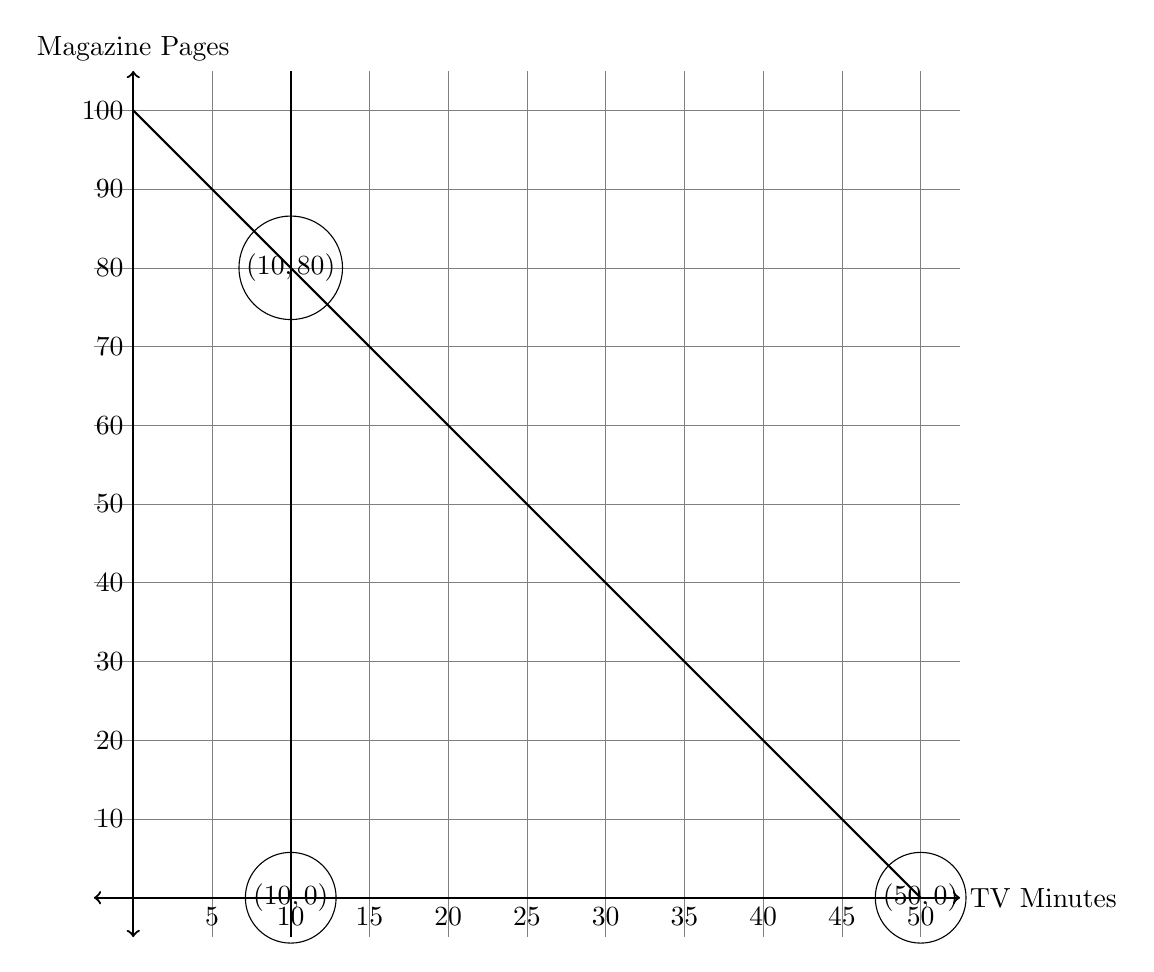
\begin{tikzpicture}
\draw[help lines] (-0.5,-0.5) grid (10.5,10.5);
\draw[thick][<->](0,10.5)--(0,-0.5);
\draw (0,10.5) node[above]{Magazine Pages};
\draw[thick][<->](10.5,0)--(-.5,0);
\draw (10.5,0) node[right]{TV Minutes};
\draw (0,1) node[left]{10};
\draw (0,2) node[left]{20};
\draw (0,3) node[left]{30};
\draw (0,4) node[left]{40};
\draw (0,5) node[left]{50};
\draw (0,6) node[left]{60};
\draw (0,7) node[left]{70};
\draw (0,8) node[left]{80};
\draw (0,9) node[left]{90};
\draw (0,10) node[left]{100};
\draw (1,0) node[below]{5};
\draw (2,0) node[below]{10};
\draw (3,0) node[below]{15};
\draw (4,0) node[below]{20};
\draw (5,0) node[below]{25};
\draw (6,0) node[below]{30};
\draw (7,0) node[below]{35};
\draw (8,0) node[below]{40};
\draw (9,0) node[below]{45};
\draw (10,0) node[below]{50};
\draw[thick] (2,10.5)--(2,-.50);
\draw[thick] (0,10)--(10,0);
\draw [nodes=draw, circle, inner sep=1.5pt]
    (2,8) node [] {$(10,80)$}
	(2,0) node []{$(10,0)$}
	(10,0) node [] {$(50,0)$};
\end{tikzpicture}

We see the corner points of the feasible set as possible solutions.  We are left to find the maximum:

\begin{tabular}{c|c|c}
Point& z & Optimizer\\\hline
$(10,80)$& 18+80 = 98&Max\\
$(10,0)$& 18+0 = 18&Min\\
$(50,0)$& 90+0 = 90&
\end{tabular}
We repeat the same system in AMPL and arrive at the same solution

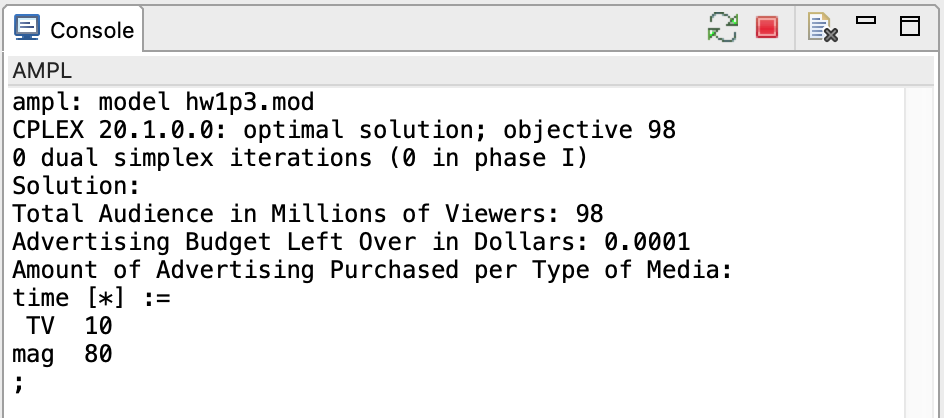
\includegraphics{outputp3a.png}
\item For this part, we repeat the exercise adding the additional requirement of creative time
\[
1x+3y\leq 100
\]
We see this changes our maximum, to 92 million people.

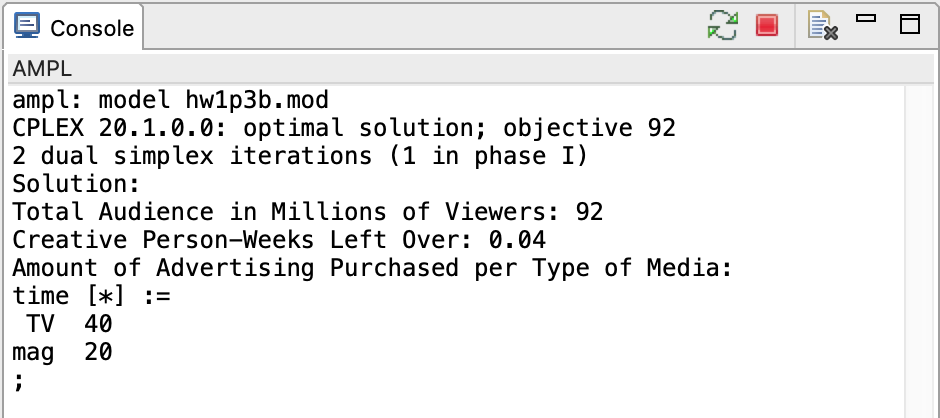
\includegraphics{outputp3b.png}

\item For the next question we add radio into the advertising mix.  This will add a new variable and change all the constraints and objective.  We also note that the 2D graphical method will no longer be available to us to check our solution.
\[
z =  1.8 x_{TV} + 1x_{magazine} + 0.25x_{radio}
\]
\[
\begin{array}{l}
x_{TV}\geq 10\\
20 000 x_{TV} + 10 000 x_{magazine} + 2 000 x_{radio} \leq 1 000 000\\
1x_{TV}+3x_{magazine} + 1 x_{radio} + \leq 100
\end{array}
\]
We change notation here too, applying subscripts to be more descriptive of our vector $x$.

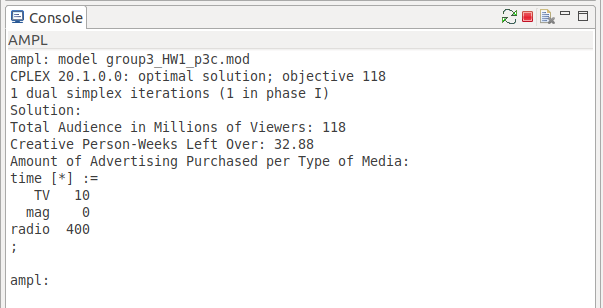
\includegraphics{outputp3c.png}

We should take a moment to examine this solution.  It slightly increases our total number of customers 93.89 million but includes no magazine advertizing.  It also requires fractional time in TV and radio.  While these are possible it is not known to the authors if this is available in the Ad world.
\item To add the condition of at lease two pages of magazine, we add the condition
\[
x_{magazine}\geq 2
\]
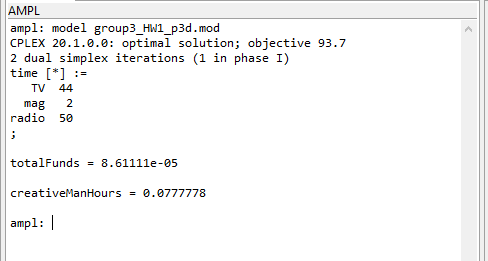
\includegraphics{outputp3d1.png}

We can add the requirement of no more that 120 minutes of radio but that will not change the results.  We include that constraint for completeness and rerun similar code to above.
\[
x_{radio} \leq 120
\]
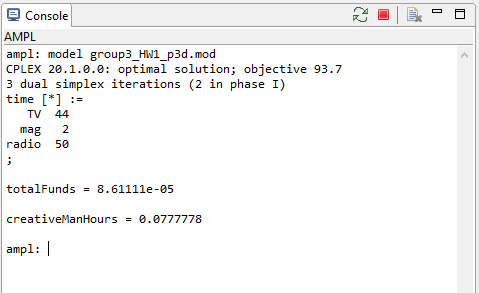
\includegraphics{outputp3d2.png}

We should note that viewership numbers are high with this model and there are no fractional pages or minutes required to achieve this solution
\end{enumerate}

\item We'll repeat the question here
\begin{quote}
The steel model of this chapter can be further modified to reflect various changes in production requirements. For each part below, explain the modifications to Figures 1-6a and 1-6b that
would be required to achieve the desired changes. (Make each change separately, rather than accumulating the changes from one part to the next.)

\begin{enumerate}
\item How would you change the constraints so that total hours used by all products must equal the total hours available for each stage? Solve the linear program with this change, and verify that you
get the same results. Explain why, in this case, there is no difference in the solution.
\item How would you add to the model to restrict the total weight of all products to be less than a
new parameter, max\_weight? Solve the linear program for a weight limit of 6500 tons, and
explain how this extra restriction changes the results.
\item The incentive system for mill managers may tend to encourage them to produce as many tons as
possible. How would you change the objective function to maximize total tons? For the data of
our example, does this make a difference to the optimal solution?
\item Suppose that instead of the lower bounds represented by commit[p] in our model, we want to
require that each product represent a certain share of the total tons produced. In the algebraic notation of Figure 1-1, this new constraint might be represented as
\[
X_j \geq s_j\sum_{k\in P} X_k, \forall j \in P
\]
where s j is the minimum share associated with project j. How would you change the AMPL model
to use this constraint in place of the lower bounds commit[p]? If the minimum shares are 0.4 for
bands and plate, and 0.1 for coils, what is the solution?  Verify that if you change the minimum shares to 0.5 for bands and plate, and 0.1 for coils, the linear program gives an optimal solution that produces nothing, at zero profit. Explain why this makes sense.
\item Suppose there is an additional finishing stage for plates only, with a capacity of 20 hours and a
rate of 150 tons per hour. Explain how you could modify the data, without changing the model, to
incorporate this new stage.
\end{enumerate}
\end{quote}

\begin{enumerate}
\item To make the constraint from a less than to equal, we simply change the constraint in AMPL to $==$ instead of $<=$.  We see a screen shot of this in the code base:

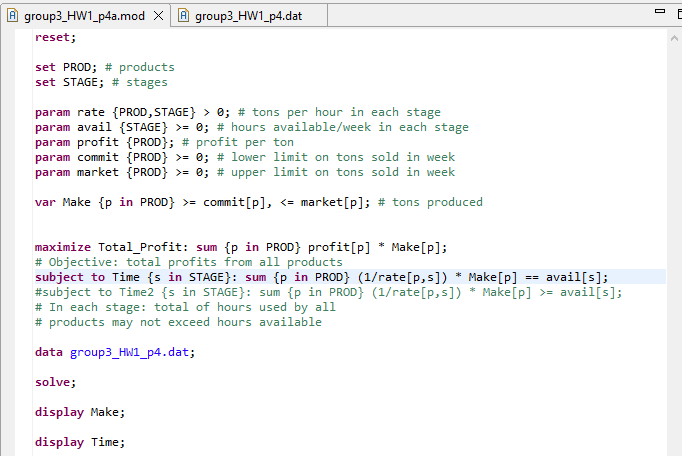
\includegraphics[width = \textwidth]{outputp4a1.png}

We see that the output agrees with the values reported in the text.

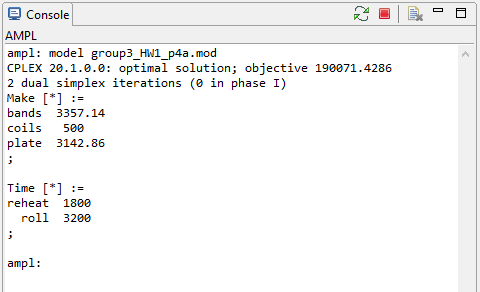
\includegraphics{outputp4a2.png}

The reason for this agreement even with a new condition is that we were already using all available hours.  It did not matter that we required equality as it was already achieved in the optimizer.
\item Adding the constraint of max\_weight will result in an extra constraint.  Using the language of text, we will require that
\[
\sum_{p \in PROD}Make[p] \leq max\_weight
\]
When added to our model we see the following results

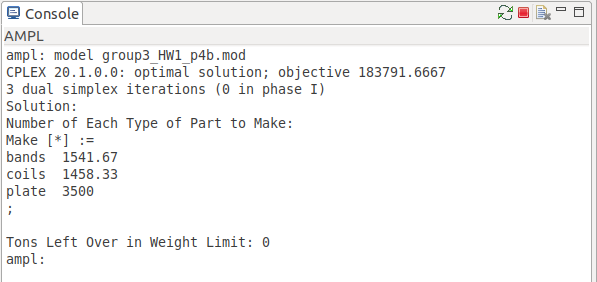
\includegraphics{outputp4b.png}

We note that the objective has dropped with this production schedule and there are still more than 13 tons left that could have been assembled in this new weight limit scenario.  We can also see that the original optimizer was over this weight limit which is why we now have a new result.

\item To examine this question, we change the objective function.  We now which to maximize the total weight produced rather than the profit.  The new objective is simply
\[
z = \sum_{i\in PROD} x_i
\]
We make this the sole objective in the system in AMPL and provide the Total\_Profit for comparison.

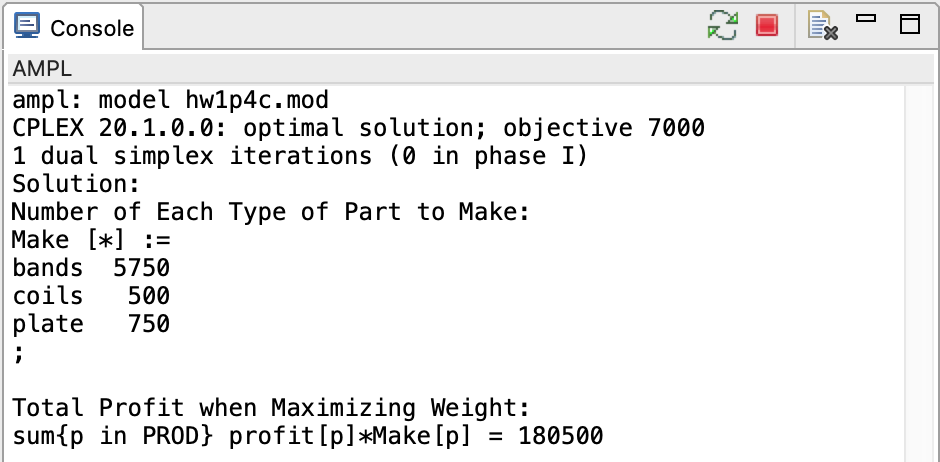
\includegraphics{outputp4c.png}

We note that the profit has dropped (as expected) but the total weight did not actually change from the original result, both are 7000 tonnes.

\item To tackle this question, we first restate the question in our own terms.  Here we desire not a baseline production but a baseline production percentage.  In reality what we desire is a minimum percentage of the total to be in each product.  We will make this a separate constraint called Production\_Percentage and eliminate the commit minimums.  We write the percentage as a new param and write the constraint as 
\[
\text{subject to percentage} \{p \in PROD\}: Make[p] \geq percent[p]*\left(sum \{r \in PROD\} Make[r]\right);
\]
Output is included below and shows that constraint decreases the optimal profit.

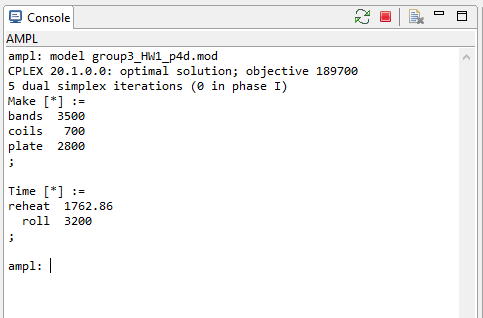
\includegraphics{outputp4d.png}

If we change the percentages to 50\% for two products and 10\% for the remaining we indeed produce nothing.  Afterall the only way give 110\% is to have started with nothing...

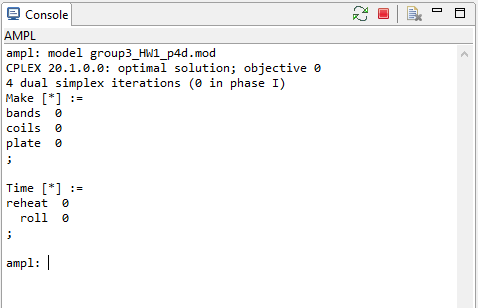
\includegraphics{outputp4d1.png}

\item Something, something add hours and change a rate... \LaTeX 

\hrule

\end{enumerate}
\item We restate the question here:

\begin{quote}
Consider the bond-portfolio problem formulated in Section 1.3 (in this assignment question 2). Reformulate the problem restricting the bonds available only to bonds A and D. Further add a constraint that the holdings of municipal bonds must be less than or equal to \$3 million.
\begin{enumerate}
\item What is the optimal solution?
\item What is the shadow price on the municipal limit?
\item How much can the municipal limit be relaxed before it becomes a nonbinding constraint?
\item Below what interest rate is it favorable to borrow funds to increase the overall size of the portfolio?
\item Why is this rate less than the earnings rate on the portfolio as a whole?
\end{enumerate}
\end{quote}
\begin{enumerate}
\item Since bond $A$ was the only remaining Municipal bond, the only new constraint is
\[
invest[A] \leq 3 000 000
\]
We copy/pasta the data file from question 2 and delete all mentions to bond $E$ as well.  Output is shown below.

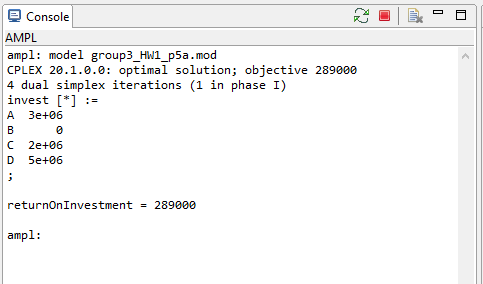
\includegraphics{outputp5a.png}

\item To find the shadow price on the municipal limit we simply increase the limit by \$1 and see how the optimal value changes.  This change in the optimal value is the shadow price.  We see in the output below some interesting features by this slight change.  First off, the objective (profit) has increased by \$0.003 but the investment strategy changed the amount invested in Bond $C$ decreasing it by \$10.  We are unsure where that extra money was to be invested due to other outputs expressed in scientific notation.  This shadow price was also observed to be the same if we added another dollar to the constraint or subtracted a dollar!

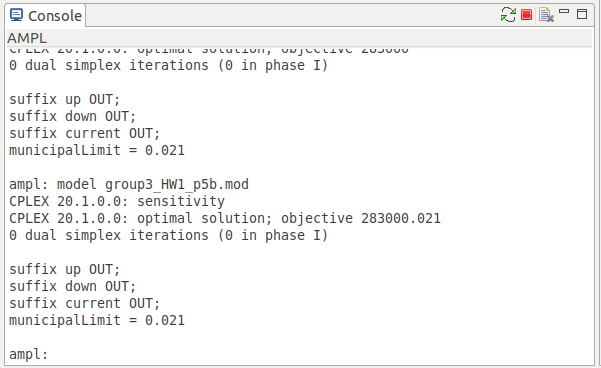
\includegraphics{outputp5b.png}

We note that after videos dropped explaining how to compute shadow limit with AMPL, we repeated this exercise using the cplex\_options 'sensitivity' and found the same result presented below.

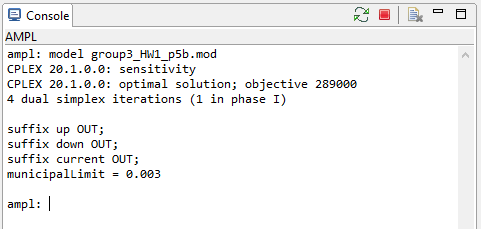
\includegraphics{outputp5bwOption.png}
\item To see how much this municipal constraint can be relaxed before becoming non-binding, we simply increased the limit to \$4 000 000.  When we run the code with that limit, we see that we do not achieve that limit but instead have a limit in bond $A$ of \$ 3 333 330.  We wonder if the actual value should be \$ 3 333 333.3$\overline{3}$.

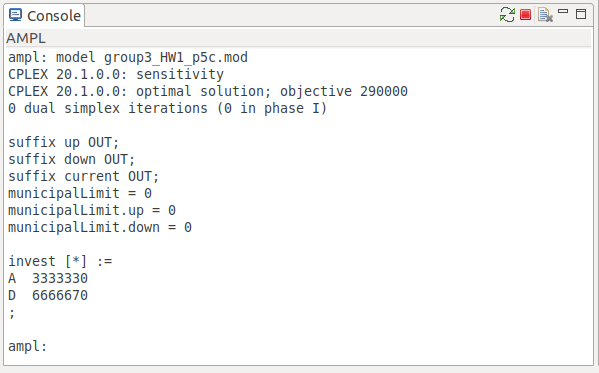
\includegraphics{outputp5c.png}

\item Something about tax rates....

\item Because of constraints on ratings and time to maturity. 
\end{enumerate}
\end{enumerate}



\end{document}